\documentclass[10pt]{beamer}

\usetheme{Warsaw}
\beamertemplatenavigationsymbolsempty

\usepackage[utf8]{inputenc}
\usepackage[francais]{babel}
\usepackage{hyperref}
\usepackage{amsmath}
\usepackage{graphicx}
\graphicspath{{./img/}}
\DeclareGraphicsExtensions{.png, .jpeg, .jpg}


\renewcommand*\thesection{\arabic{section}}


\AtBeginSection[]{%
  \begin{frame}<beamer>
    \frametitle{Plan}
    \tableofcontents[sectionstyle=show/hide,subsectionstyle=hide/show/hide]
  \end{frame}
  \addtocounter{framenumber}{-1}
}



\title{Obtention efficace des Longest Common Prefixes}
\author{Rémi Bois, Loïc Jankowiac}
\date{\today}

\begin{document}

\begin{frame}
  \maketitle

\end{frame}

\begin{frame}
  \tableofcontents
\end{frame}

\section{Contexte}
\label{sec:context}



\begin{frame}
  \frametitle{Recherche de pattern à partir d'un tableau des suffixes
    et des longest common prefixes}
  %description de l'efficacité de la recherche via le tableau des
  %suffixes en termes de complexité algorithmique et spaciale

  \begin{block}{arbre des suffixes vs tableau des suffixes} 
    Le tableau des suffixes est une représentation compacte de l'arbre
    des suffixes. Le principal avantage du tableau des suffixes comparé à
    l'arbre des suffixes est la place mémoire occuppée, environ 4 fois
    moins importante. Cette contrainte est importante lors de
    recherche sur de longs textes, notamment en bioinformatique \cite{Raffinot11}.
  \end{block}

  \pause

  \begin{block}{La recherche de motifs}
    Le tableau des suffixes permet de trouver les occurrences d'un
    motif dans un texte en $O(m*log(n))$. Associé aux informations sur
    les plus longs préfixes communs (Longest Common Prefixes,
    \emph{lcp}), il permet une recherche en $O(m + log(n))$ \cite{Manber93}.
  \end{block}
  
\end{frame}

\begin{frame}
  \frametitle{Quelques notations}
  %lcp, A, et tout ce dont on aura besoin dans sec:algo
  On utilisera les notation suivantes :

  \begin{itemize}
  \item lcp : Longest Common Prefixes
  \item A : un texte et $A_i$ le suffixe de A commençant à la position i.
  \item S : la sous-chaîne (motif) recherché dans le texte A.
  \item $Occ(S, A)$ : l'ensemble des occurrences de S dans A.
  \end{itemize}
\end{frame}

\begin{frame}
  \frametitle{Un élément manquant : les longest common prefixes}
  %cadre dans lequel on se place : on a le texte et le tableau des
  %suffixes. Il manque les lcp pour faire une recherche efficace
  Dans les faits, le calcul des lcp se fait lors de la construction de
  l'arbre des suffixes, ou du tableau des suffixes. Il ne rajoute pas
  de complexité à ces constructions (l'ordre de grandeur reste
  identique).

  L'article présenté propose un moyen efficace d'obtenir
  les informations des lcp lorsque celles-ci ne sont pas
  disponibles\cite{Kasai01}.
\end{frame}


\begin{frame}
  \frametitle{Un contexte réaliste ?}
  %intro sur les deux problèmes qu'on explorera plus tard
  Un algorithme de compression basé sur la transformation de
  Burrow-Wheeler \cite{Burrows94}, très utilisé (\emph{bizp2}), permet
  de retrouver, lors de la décompression, le tableau des suffixes. 

  Il ne manque alors plus que les informations sur les lcps pour faire
  une recherche efficace. 
\end{frame}

\section{Calculer les lcps en O(n)}
\label{sec:algo}

%Faut voir comment on organise ça. Faut le faire tourner sur un
%exemple (abraca ?)


\section{Application à la recherche de pattern dans un texte compressé}
\label{sec:appcompress}

\begin{frame}
  \frametitle{La compression par Block-Sorting}
  %complexité, implémentations

  \begin{block}{Un bon compromis}
    Block-sorting parvient à obtenir un très bon taux de compression
    tout en étant rapide (vitesse proche de LZ et compression proche
    des modèles statistiques\cite{Burrows94}).
  \end{block}

  \begin{block}{Basée sur une idée ``simple''}
    Le but est de rapprocher les caractères identiques d'un texte et
    d'utiliser un encodage ``move-to-front'' consistant à indiquer la
    distance du prochain caractère identique. On utilise ensuite un
    codage de Huffman pour encoder la suite obtenue.
  \end{block}


\end{frame}

\begin{frame}
  \frametitle{Comment ça marche ?}
  %exemple sur abcabbca$. On s'arrête après la rotation et l'obtention de
  %L, I. On explique "grossièrement" la suite (en une dizaine de
  %secondes)
  \begin{figure}
    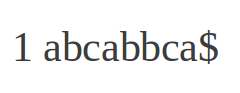
\includegraphics[width=0.22\textwidth]{start_burrows}
  \end{figure}

\end{frame}

\begin{frame}
  \frametitle{Comment ça marche ?}
  %exemple sur abcabbca$. On s'arrête après la rotation et l'obtention de
  %L, I. On explique "grossièrement" la suite (en une dizaine de
  %secondes)
  \begin{figure}
    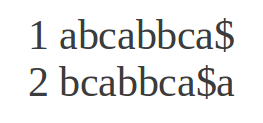
\includegraphics[width=0.21\textwidth]{1_burrows}
  \end{figure}

\end{frame}

\begin{frame}
  \frametitle{Comment ça marche ?}
  %exemple sur abcabbca$. On s'arrête après la rotation et l'obtention de
  %L, I. On explique "grossièrement" la suite (en une dizaine de
  %secondes)
  \begin{figure}
    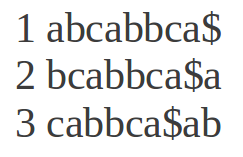
\includegraphics[width=0.2\textwidth]{2_burrows}
  \end{figure}

\end{frame}

\begin{frame}
  \frametitle{Comment ça marche ?}
  %exemple sur abcabbca$. On s'arrête après la rotation et l'obtention de
  %L, I. On explique "grossièrement" la suite (en une dizaine de
  %secondes)
  \begin{figure}
    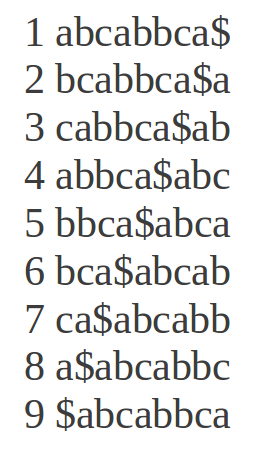
\includegraphics[width=0.2\textwidth]{3_burrows}
  \end{figure}

\end{frame}

\begin{frame}
  \frametitle{Comment ça marche ?}
  %exemple sur abcabbca$. On s'arrête après la rotation et l'obtention de
  %L, I. On explique "grossièrement" la suite (en une dizaine de
  %secondes)
  \begin{figure}
    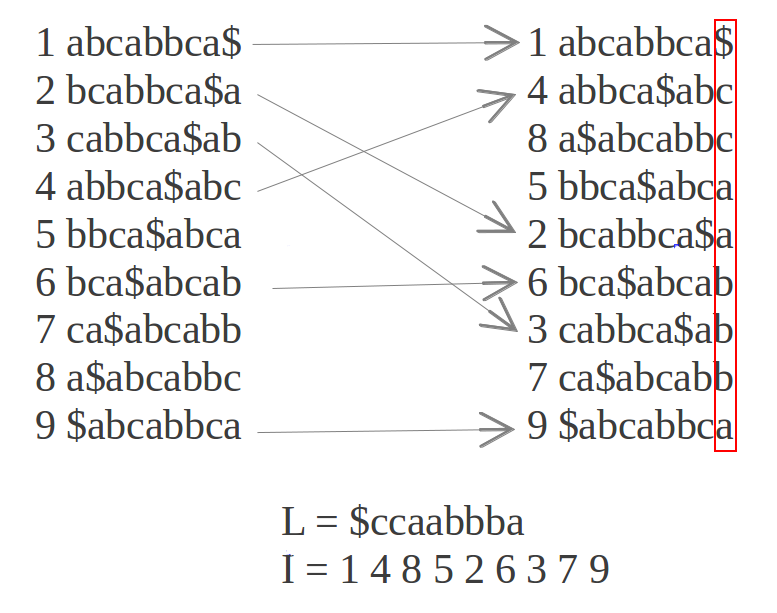
\includegraphics[width=0.5\textwidth]{full_burrows}
  \end{figure}

\end{frame}

\begin{frame}
  \frametitle{Pourquoi ça nous intéresse ?}
  %on peut retrouver le tableau des suffixes à partir de L, I mais il
  %nous manque les informations sur les LCPs. On peut les retrouver en
  %O(n).

  \begin{block}{Comme un air de famille entre I et Pos}
    Le tableau I est en fait le tableau des suffixes.
    Il ne manque donc plus que les informations sur les lcp pour faire
    une recherche efficace.
  \end{block}

\end{frame}

%Une conclusion à cette section ?


\section{Simulation d'un parcours bottom-up de l'arbre des suffixes}
\label{sec:appbottomup}

%Aucune idée pour l'instant. Pas sûr qu'on aura le temps de présenter
%en détail cette section.

\section{Conclusion}
\label{sec:conclusion}

\begin{frame}
  \frametitle{Un algorithme performant et simple}
  %rappel de la complexité, des cas d'utilisations, ...
\end{frame}

\begin{frame}
  \frametitle{Des questions ?}
  %une image sympa
\end{frame}

\begin{frame}
  \frametitle{Références}
  %les articles cités
  \bibliographystyle{amsalpha}
  \bibliography{./pres.bib}
\end{frame}

\end{document}